\label{repr_mat_red_dist_interat}

\subsection{Motivation}

\label{repr_mat_red_dist_interat_motiv}

\par Cette représentation est issue du travail qui a été fait précédemment sur ce projet, et consiste à représenter une molécule par ses distances inter-atomiques. L'intérêt de cette représentation est que les réseaux de neurones qui l'utilisent travaillent dans des repères relatifs. Lorsqu'ils effectuent des prédictions, ils n'ont pas besoin d'utiliser les notions mathématiques de géométrie permettant de déduire la position d'un point dans un repère à partir de ses distances à d'autres points. Cette représentation est donc très commode pour les modèles prédictifs dont l'objectif est de corriger les distances entre deux atomes, puisqu'elle est basée sur les distances entre les paires d'atomes.

\par De plus, cette représentation offre la propriété intéressante d'être insensible aux translations de repère. En effet, deux molécules dont les distances entre chaque couple d'atomes sont identiques mais dont les atomes ne sont pas placés aux mêmes coordonnées partageront la même représentation.\\

\par Lorsque les modèles utilisent cette représentation en sortie, ou plus précisément que l'on déduit la matrice réduite des distances inter-atomiques de la sortie du modèle (\ref{delta_dist_entree_sortie}), nous devons toutefois trouver une méthode (\ref{repr_mat_dist_rel_interat_reconstruct}) pour reconstruire les molécules sous la forme d'une matrice de coordonnées (\ref{repr_mat_coords}).

\subsection{Formalisation}

\par Pour ne pas surcharger les modèles d'information, nous ne travaillons pas sur la matrice de distances inter-atomiques complète, mais sur un sous-ensemble de cardinalité minimale de cette matrice telle que nous pouvons reconstruire sans ambiguïté un ensemble de coordonnées représentant les positions des atomes de la molécule. La matrice des distances étant symétrique et la diagonale étant nulle, toute l'information est contenue dans chaque demi-matrice triangulaire privée de la diagonale. \\

\par De plus, nous n'avons besoin que des distances à quatre points pour retrouver la position de chaque atome (\ref{repr_mat_dist_rel_interat_reconstruct}), nous nous contentons donc de garder les quatre premières distances de chaque ligne de la matrice triangulaire supérieure privée de la diagonale. Une représentation générale de la matrice réduite des distances inter-atomiques est disponible dans les tableaux \ref{table_mat_interat_1} et \ref{table_mat_interat_2}.


\begin{table}
	\centering
	
	
	\begin{tabular}{c|c|c|c|c|c|c|c|c|c|c|c|c}
	    & a\textsubscript{0} & a\textsubscript{1} & a\textsubscript{2} & a\textsubscript{3} & a\textsubscript{4} & ... & a\textsubscript{n-4} & a\textsubscript{n-3} & a\textsubscript{n-2} & 
	    	 a\textsubscript{n-1}  & a\textsubscript{n}\\ \hline
		a\textsubscript{0} & d\textsubscript{0,0} & \textbf{d\textsubscript{0,1}} & \textbf{d\textsubscript{0,2}} & 
		    \textbf{d\textsubscript{0,3}} & \textbf{d\textsubscript{0,4}} & ... & d\textsubscript{0,n-4} & 
		    d\textsubscript{0,n-3} & d\textsubscript{0,n-2} & d\textsubscript{0,n-1}
		    & d\textsubscript{0,n} \\ \hline
		a\textsubscript{1} & d\textsubscript{1,0} & d\textsubscript{1,1} & \textbf{d\textsubscript{1,2}} & 
			\textbf{d\textsubscript{1,3}} & \textbf{d\textsubscript{1,4}} & ... & d\textsubscript{1,n-4} & 
			d\textsubscript{1,n-3} & d\textsubscript{1,n-2} & d\textsubscript{1,n-1} & 
			d\textsubscript{1,n} \\ \hline
		a\textsubscript{2} & d\textsubscript{2,0} & d\textsubscript{2,1} & d\textsubscript{2,2} &
			\textbf{d\textsubscript{2,3}} & \textbf{d\textsubscript{2,4}} & ... & d\textsubscript{2,n-4} & 
			d\textsubscript{2,n-3} & d\textsubscript{2,n-2} & d\textsubscript{2,n-1} & 
			d\textsubscript{2,n} \\ \hline
		a\textsubscript{3} & d\textsubscript{3,0} & d\textsubscript{3,1} & d\textsubscript{3,2} & 
			d\textsubscript{3,3} & \textbf{d\textsubscript{3,4}} & ... & d\textsubscript{3,n-4} & 
			d\textsubscript{3,n-3} & d\textsubscript{3,n-2} & d\textsubscript{3,n-1} & 
			d\textsubscript{3,n} \\ \hline
			
		a\textsubscript{4} & d\textsubscript{4,0} & d\textsubscript{4,1} & d\textsubscript{4,2} & 
			d\textsubscript{4,3} & \textbf{d\textsubscript{4,4}} & ... & d\textsubscript{4,n-4} & 
			d\textsubscript{4,n-3} & d\textsubscript{4,n-2} & d\textsubscript{4,n-1} & 
			d\textsubscript{4,n} \\ \hline
			
		\rot{... } & \rot{... } & \rot{... } & \rot{... } & \rot{... } & 
		\rot{... } & \halfrot{ ... } & \rot{... } & \rot{... } & \rot{... } & 
		\rot{... } & \rot{... } \\ \hline
	    	
	    	
		a\textsubscript{n-4} & d\textsubscript{n-4,0} & d\textsubscript{n-4,1} & d\textsubscript{n-4,2} & 
			d\textsubscript{n-4,3} & d\textsubscript{n-4,4} & ... & d\textsubscript{n-4,n-4} & 
			\textbf{d\textsubscript{n-4,n-3}} & \textbf{d\textsubscript{n-4,n-2}} & \textbf{d\textsubscript{n-4,n-1}} & 
			\textbf{d\textsubscript{n-4,n}} \\ \hline	    
		a\textsubscript{n-3} & d\textsubscript{n-3,0} & d\textsubscript{n-3,1} & d\textsubscript{n-3,2} & 
			d\textsubscript{n-3,3} & d\textsubscript{n-3,4} & ... & d\textsubscript{n-3,n-4} & 
			d\textsubscript{n-3,n-3} & \textbf{d\textsubscript{n-3,n-2}} & \textbf{d\textsubscript{n-3,n-1}} & 
			\textbf{d\textsubscript{n-3,n}} \\ \hline
		a\textsubscript{n-2} & d\textsubscript{n-2,0} & d\textsubscript{n-2,1} & d\textsubscript{n-2,2} & 
			d\textsubscript{n-2,3} & d\textsubscript{n-2,4} & ... & d\textsubscript{n-2,n-4} & 
			d\textsubscript{n-2,n-3} & d\textsubscript{n-2,n-2} & \textbf{d\textsubscript{n-2,n-1}} & 
			\textbf{d\textsubscript{n-2,n}} \\ \hline
		a\textsubscript{n-1} & d\textsubscript{n-1,0} & d\textsubscript{n-1,1} & d\textsubscript{n-1,2} & 
			d\textsubscript{n-1,3} & d\textsubscript{n-1,4} & ... & d\textsubscript{n-1,n-4} & 
			d\textsubscript{n-1,n-3} & d\textsubscript{n-1,n-2} & d\textsubscript{n-1,n-1} & 
			\textbf{d\textsubscript{n-1,n}} \\ \hline
		a\textsubscript{n} & d\textsubscript{n,0} & d\textsubscript{n,1} & d\textsubscript{n,2} & 
			d\textsubscript{n,3} & d\textsubscript{n,4} & ... & d\textsubscript{n,n-4} & 
			d\textsubscript{n,n-3} & d\textsubscript{n,n-2} & d\textsubscript{n,n-1} & d\textsubscript{n,n} \\ \hline
		
	\end{tabular}

	
	\caption{Matrice réduite des distances inter-atomiques d'une molécule (en gras), au sein de la matrice complète des distances inter-atomiques}
	\label{table_mat_interat_1}

\end{table}

\begin{table}
	\centering
	
	
	\begin{tabular}{|c|c|c|c|}
		\hline
		\textbf{d\textsubscript{0,1}} & \textbf{d\textsubscript{0,2}} & \textbf{d\textsubscript{0,3}} & \textbf{d\textsubscript{0,4}} \\ \hline
		\textbf{d\textsubscript{1,2}} & \textbf{d\textsubscript{1,3}} & \textbf{d\textsubscript{1,4}} & \textbf{d\textsubscript{1,5}} \\ \hline
		\textbf{d\textsubscript{2,3}} & \textbf{d\textsubscript{2,4}} & \textbf{d\textsubscript{2,5}} & \textbf{d\textsubscript{2,6}} \\ \hline
		\textbf{d\textsubscript{3,4}} & \textbf{d\textsubscript{3,5}} & \textbf{d\textsubscript{3,6}} & \textbf{d\textsubscript{3,7}} \\ \hline
		\textbf{\rot{... }} & \textbf{\rot{... }} & \textbf{\rot{... }} & \textbf{\rot{... }} \\ \hline
		\textbf{d\textsubscript{n-4,n-3}} & \textbf{d\textsubscript{n-4,n-2}} & \textbf{d\textsubscript{n-4,n-1}} & \textbf{d\textsubscript{n-4,n}} \\ \hline
		\textbf{d\textsubscript{n-3,n-2}} & \textbf{d\textsubscript{n-3,n-1}} & \textbf{d\textsubscript{n-3,n}} & \textbf{0} \\ \hline
		\textbf{d\textsubscript{n-2,n-1}} & \textbf{d\textsubscript{n-2,n}} & \textbf{0} & \textbf{0} \\ \hline
		\textbf{d\textsubscript{n-1,n}} & \textbf{0} & \textbf{0} & \textbf{0} \\ \hline
	\end{tabular}

	
	\caption{Matrice réduite des distances inter-atomiques d'une molécule}
	\label{table_mat_interat_2}
\end{table}

\newpage
\subsection{Reconstruction des molécules}

\label{repr_mat_dist_rel_interat_reconstruct}

\par Lorsqu'un modèle a pour sortie une matrice réduite des distances inter-atomiques, il faut définir une méthode pour reconstruire une matrice des coordonnées (\ref{repr_mat_coords}) de façon automatique à partir de cette sortie, la seule contrainte étant que la distance relative entre chaque paire d'atomes soit respectée. Il ne s'agit pour autant pas d'une tâche triviale. Elle s'est en effet avérée impossible en pratique pour les grosses molécules à cause de la propagation des erreurs qu'elle induit (\ref{repr_mat_dist_rel_interat_trilat}).

\subsubsection{Formalisation de la méthode de reconstruction}

\label{repr_mat_dist_rel_interat_form_reconstruct}

\paragraph{Nécessité et limite de l'introduction d'un atome fictif} Notre méthode de reconstruction des atomes doit permettre de respecter la chiralité\footnote{Un composé chimique est dit chiral s'il n'est pas superposable à son image dans un miroir. (https://fr.wikipedia.org/wiki/Chiralité\_(chimie)} des molécules. Or, en déduisant uniquement la position d'un atome de ses distances aux quatre atomes précédents, il existe des cas pour lesquels il existe plusieurs solutions pour la position de l'atome (deux si les quatre atomes précédents sont sur un même plan, ou une infinité si les quatre atomes précédents appartiennent à une droite). Pour pallier ce problème, la méthode retenue lors des stages précédents a été d'introduire un nouveau point (que l'on nomme atome fictif) et que l'on place arbitrairement dans la molécule, à une position telle qu'il n'appartient pas au plan formé par les trois premiers atomes, ni à la droite formée par les trois premiers atomes s'ils sont alignés. De cette façon, les atomes suivants seront placés sans ambiguïté.\\
Cependant, on peut imaginer des cas pour lesquels la technique de l'introduction d'un atome fictif ne permet pas de lever l'ambiguïté, notamment pour les molécules possédant une chaîne d'atomes formant une droite. La méthode ne permettra pas dans ce cas de déterminer les positions des atomes en bout de chaîne, cette information étant perdue lors de la création de la matrice réduite des distances inter-atomiques. \\
Cette représentation n'est donc pas viable en pratique. Cela fait partie des raisons (voir également \ref{repr_mat_dist_rel_interat_trilat}) pour lesquelles nous sommes passés à la représentation par matrice réduite des distances à des points fixes (\ref{repr_mat_pts_fixes}).

\paragraph{Placement de l'atome fictif} Puisque l'on définit la position de chaque atome en fonction de ses distances aux quatre atomes précédents, on doit d'abord placer les quatre premiers atomes de façon partiellement arbitraire. Le premier atome de la molécule dans notre représentation étant l'atome fictif a\indice{0}, nous commençons par le placer à la position qui lui a été attribuée.

\paragraph{Placement de l'atome a\indice{1}} Une fois l'atome a\indice{0} placé, il existe une infinité de solutions pour la position de l'atome a\indice{1}. On peut en effet le placer à tout point appartenant à la surface de la sphère de centre a\indice{0} et de rayon d\indice{0,1}. L'ensemble des solutions est visible dans la figure \ref{fplacement_a1}.

\begin{figure}
	\centering
	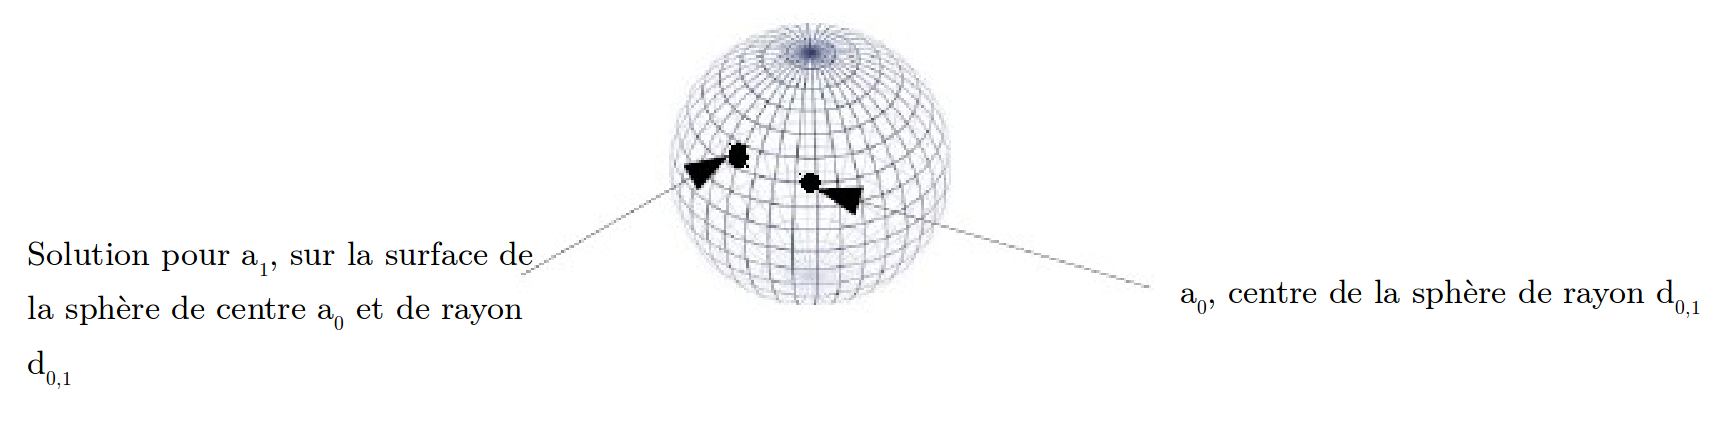
\includegraphics[scale=0.27]{images/1_sphere.png}
	\caption{Placement de l'atome a\indice{1} (image extraite du rapport de N.Roux)}
	\label{fplacement_a1}
\end{figure}

\paragraph{Placement de l'atome a\indice{2}} L'atome a\indice{2} appartient au cercle solution de l'intersection entre les sphères de centres a\indice{0} et a\indice{1} et de rayons d\indice{0,2} et d\indice{1,2}. On choisit donc arbitrairement une position appartenant à ce cercle. L'ensemble des solutions est visible dans la figure \ref{fplacement_a2}.

\begin{figure}
	\centering
	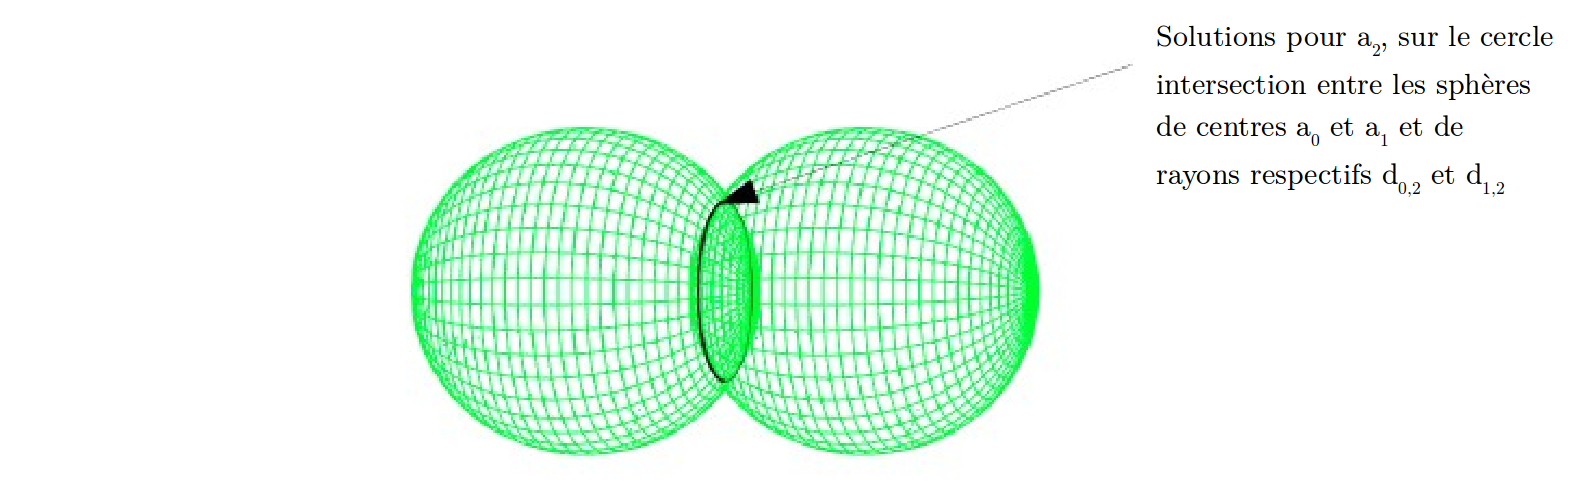
\includegraphics[scale=0.3]{images/2_spheres.png}
	\caption{Placement de l'atome a\indice{2} (image extraite du rapport de N.Roux)}
	\label{fplacement_a2}
\end{figure}


\paragraph{Placement de l'atome a\indice{3}} Dans le cas général, il existe deux solutions pour le placement de l'atome a\indice{3}, l'intersection non nulle de trois sphères étant deux points si tous les points ne sont pas sur un même plan ou une même droite. On choisit arbitrairement un point parmi ces deux solutions, car il n'y a pas à ce stade d'ambiguïté de chiralité de la molécule. Une molécule composée de trois atomes ne posséde en effet pas de chiralité (l'atome fictif a\indice{0} ne fait pas partie de la molécule).  L'ensemble des solutions est visible dans la figure \ref{fplacement_a3}.


\begin{figure}
	\centering
	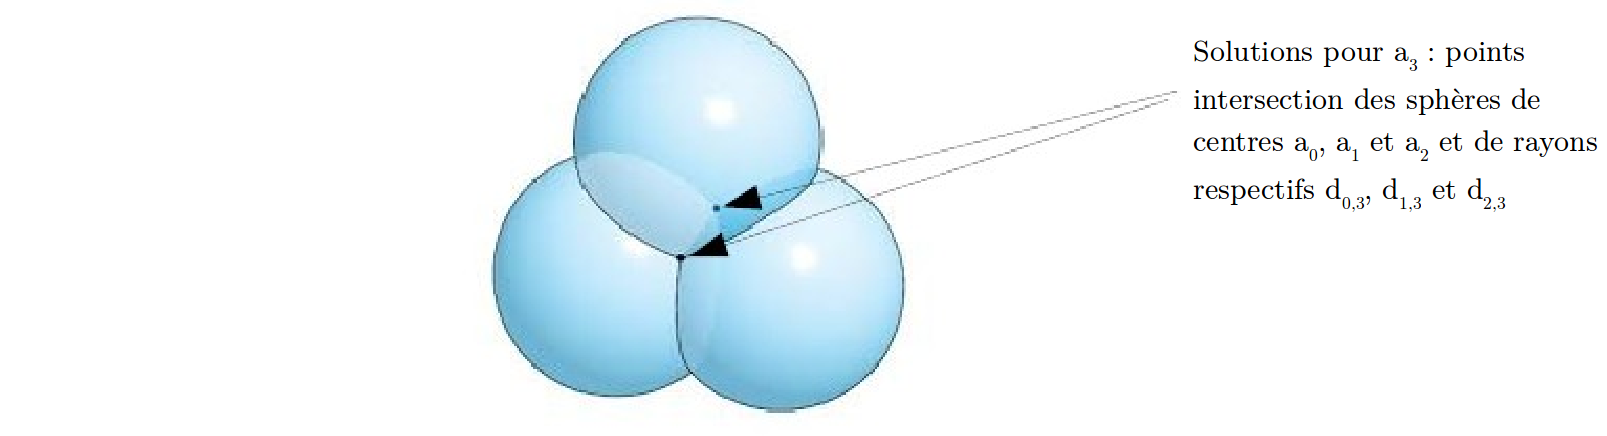
\includegraphics[scale=0.3]{images/3_spheres.png}
	\caption{Placement de l'atome a\indice{3} (image extraite du rapport de N.Roux)}
	\label{fplacement_a3}

\end{figure}



\paragraph{Placement de l'atome a\indice{n}} Pour placer l'atome a\indice{$n$} ($n$ étant inférieur à la taille de la molécule), nous généralisons la méthode de placement de l'atome a\indice{3}. Plutôt que de travailler sur l'intersection de quatre sphères, nous travaillons toujours sur l'intersection de trois sphères et nous utilisons la dernière distance pour discriminer les deux solutions obtenues. Cela facilite grandement la résolution des équations mathématiques associées et permet d'obtenir des solutions sensiblement équivalentes. \\
Formellement, nous calculons les positions des deux points solutions de l'intersection des trois sphères de centres a\indice{n-4}, a\indice{n-3}, et a\indice{n-2} et de rayons d\indice{n-4,n}, d\indice{n-3,n} et d\indice{n-2,n}, et nous discriminons les deux solutions selon la distance d\indice{n-1,n}.  L'ensemble des solutions est visible dans la figure \ref{fplacement_an}.

\begin{figure}
	\centering
	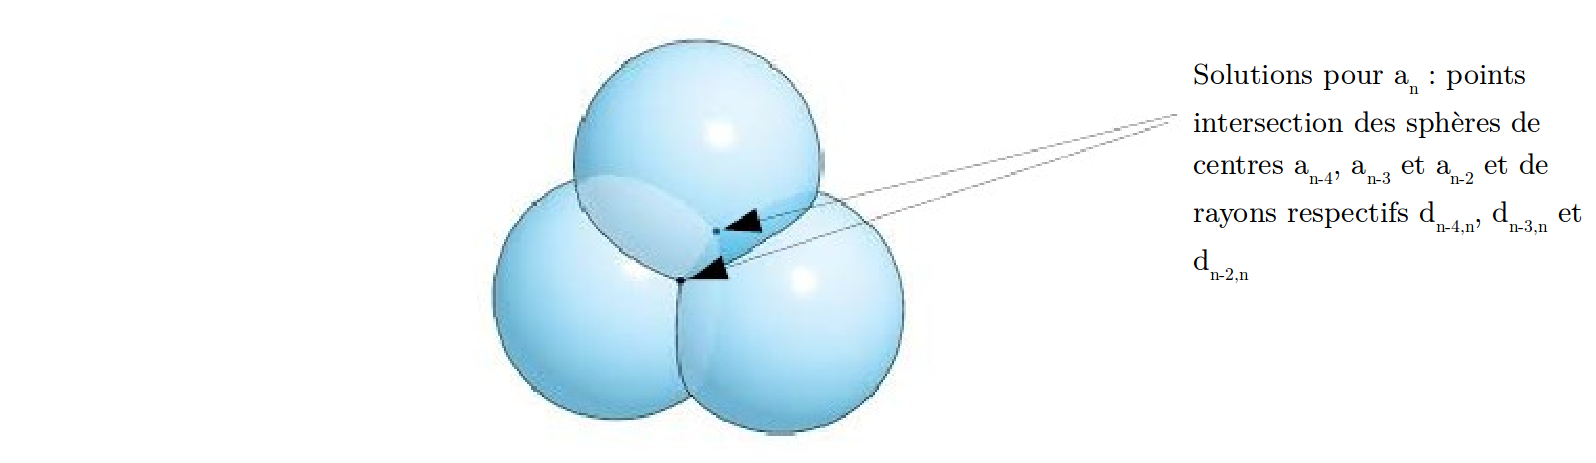
\includegraphics[scale=0.3]{images/3_spheres_gen.png}
	\caption{Placement de l'atome a\indice{n} (image extraite du rapport de N.Roux)}
	\label{fplacement_an}

\end{figure}

\subsubsection{Reconstruction automatique des positions en utilisant un solveur}

\par Nous développons ici une méthode permettant de déterminer les coordonnées d'un atome quelconque en utilisant un solveur d'équations non linéaires \footnote{https://en.wikipedia.org/wiki/Nonlinear\_system}. Nous utilisons pour cela la bibliothèque Sympy\footnote{http://www.sympy.org/fr/}.\\

\par Tout d'abord, l'atome fictif a\indice{0} doit être placé à la position qui lui a été attribuée (\ref{repr_mat_dist_rel_interat_form_reconstruct}). Nous plaçons ensuite arbitrairement les trois atomes suivants, de sorte que leurs distances relatives soient respectées. Pour simplifier le problème, nous effectuons une translation temporaire telle que a\indice{0}$'$ est à l'origine du repère. Nous plaçons alors a\indice{1}$'$ sur l'axe $x$, à une distance d\indice{0,1} de l'origine, et a\indice{2}$'$ sur le plan tel que $z=0$, à une position telle que les distances d\indice{0,2} et d\indice{1,2} sont respectées. Pour finir, nous plaçons a\indice{3}$'$ à l'une des deux solutions de l'intersection des sphères associées au problème (\ref{repr_mat_dist_rel_interat_form_reconstruct}). Le choix de la solution est arbitraire car la reconstruction de la bonne chiralité de la molécule ne dépend pas du placement des trois premiers atomes non fictifs. Les équations de placement des quatre premiers atomes sont décrites en eq. \eqref{eq_placement_a03}. \\
\begin{equation}
	a_{0}'\left \{
   	\begin{array}{l}
      x_{0}'=0\\
      y_{0}'=0\\
	  z_{0}'=0
   	\end{array}
   	\right .
   	\:
   	a_{1}'\left \{
   	\begin{array}{l}
      x_{1}'=d_{0,1}\\
      y_{1}'=0\\
	  z_{1}'=0
   	\end{array}
   	\right .
   	\:
	a_{2}'\left \{
   	\begin{array}{l}
      x_{2}'=\frac{d_{0,2}^2 - d_{1,2}^2 + x_{1}^2}{2x_{1}'}\\
      y_{2}'=\sqrt{d_{2,0}^2 - x_{2}'^2}\\
	  z_{2}'=0
   	\end{array}
   	\right .
   	\:
   	a_{3}'\left \{
   	\begin{array}{l}
      x_{3}'=\frac{d_{0,3}^2+x_1'^2-d_{1,3}^2}{2x_{1}'}\\
      y_{3}'=\frac{-2x_3'x_2'+d_{0,2}^2-d_{2,3}^2+d_{0,3}^2}{2y_2'}\\
	  z_{3}'=\sqrt{-x_3'^2-y_3'^2+d_{0,3}^2}
   	\end{array}
   	\right .
	\label{eq_placement_a03}
\end{equation}


\par Une fois que les quatre premiers atomes sont placés, nous leur appliquons une translation selon le vecteur $\vec{a_0}$, de sorte que l'atome fictif soit à sa position originale, et que les distances relatives des atomes a\indice{0}, a\indice{1}, a\indice{2} et a\indice{3} soient toujours consistantes. Nous faisons alors appel au solveur pour résoudre les équations \eqref{eq_at_quelconque}, associées au placement des autres atomes de de la molécule. Pour chaque atome, nous sélectionnons la solution respectant au mieux la distance d\indice{n-1,n} (\ref{repr_mat_dist_rel_interat_form_reconstruct}).


\begin{equation}
	\left \{
   	\begin{array}{l}
      d_{n-4,n}^2=(x_n-x_{n-4})^2 + (y_n-y_{n-4})^2 + (z_n-z_{n-4})^2\\
	  d_{n-3,n}^2=(x_n-x_{n-3})^2 + (y_n-y_{n-3})^2 + (z_n-z_{n-3})^2\\
      d_{n-2,n}^2=(x_n-x_{n-2})^2 + (y_n-y_{n-2})^2 + (z_n-z_{n-2})^2\\
   	\end{array}
   	\right .
	\label{eq_at_quelconque}
\end{equation}
	

\paragraph{Limites de l'approche par solveur} L'utilisation d'un solveur calculant les solutions au cas par cas pose deux problèmes importants. Le premier concerne les performances de la solution. En effet, la résolution des systèmes d'équations consomme beaucoup de ressources et prend donc un temps non négligeable si l'on souhaite appliquer la méthode à un grand nombre de molécules.\\
Le second problème est lié à la propagation des erreurs lors de la reconstruction (\ref{repr_mat_dist_rel_interat_trilat}). À cause du manque de précision de certaines valeurs, certaines intersections de sphères sont vides. Le solveur renvoie alors des solutions imaginaires que nous ne pouvons pas interpréter. Ce problème se manifeste avant tout sur les molécules de grande taille, mais il est impossible de déterminer une taille limite au delà de laquelle nous ne pouvons pas reconstruire les molécules. Cela implique qu'il existe des molécules que nous ne pouvons pas reconstruire, et que nous ne pouvons pas déterminer à l'avance si une molécule donnée peut être reconstruite.


\subsubsection{Reconstruction automatique des positions en utilisant des équations de trilatération}

\label{repr_mat_dist_rel_interat_trilat}

\par Afin de pallier les problèmes liés à l'utilisation d'un solveur pour construire l'ensemble des positions des atomes d'une molécule à partir de la matrice réduite des distances inter-atomiques, nous utilisons une méthode permettant de calculer les positions de chaque point à partir d'un ensemble d'équations. Cette méthode est décrite sur Wikipédia\footnote{https://en.wikipedia.org/wiki/Trilateration}. Il s'agit d'une méthode de trilatération de points, c'est à dire que l'on cherche à déterminer la position d'un point en fonction de ses distances à trois points dont les positions sont connues, par opposition à la triangulation\footnote{https://fr.wikipedia.org/wiki/Triangulation} pour laquelle on détermine la position d'un point en fonction de ses angles à des points dont les positions sont connues.\\

\par De même que pour la méthode utilisant un solveur, nous commençons par placer l'atome fictif a\indice{0} à la position qui lui a été attribuée, puis les atomes a\indice{1}, a\indice{2} et a\indice{3} de façon arbitraire telle que les distances relatives des atomes a\indice{$i$}, $i \in \{0, ..., 3\}$ sont respectées. Nous utilisons pour cela les équations \eqref{eq_placement_a03}.\\

\par Une fois les quatre premiers atomes placés, nous cherchons à placer l'atome a\indice{$n$} de la molécule en fonction de ses distances aux quatre atomes précédents. Nous calculons les solutions en considérant que $a\indice{n-4}'$ est à l'origine du repère, que $a\indice{n-3}'$ est sur l'axe $x$, et que $a\indice{n-2}'$ est sur le plan tel que $z=0$, puis nous effectuons une translation des solutions dans le système de coordonnées original. Pour cela, nous définissons les quantités et vecteurs suivants. 
\par La notation $\hat{u}$ indique un vecteur $u$ de norme 1, et nous considérons que $\overline{a_i}$ représente le vecteur allant de l'origine au point $a_i$, dans le but de simplifier l'écriture des équations.\\

\vspace{0.4cm}

\centerline{Vecteur unitaire dans la direction de $a_{n-4}$ à $a_{n-3}$ :}

\[
\hat{e_x} = \frac{\overline{a_{n-3}}-\overline{a_{n-4}}}{d_{n-4,n-3}}
\]

\vspace{0.4cm}

\centerline{Ordre de grandeur signé de la composante $x$ dans le nouveau}
\centerline{ système de coordonnées du vecteur $\overline{a_{n-4}a_{n-2}}$ : }
\[
i = \hat{e_x}\cdot(\overline{a_{n-4}}-\overline{a_{n-2}})
\]

\vspace{0.4cm}

\centerline{Vecteur unitaire dans la direction $y$ par rapport à $\hat{e_x}$:}
\[
\hat{e_y} = \frac{\overline{a_{n-2}}-\overline{a_{n-4}}-i\hat{e_x}}{\begin{Vmatrix}\overline{a_{n-2}}-\overline{a_{n-4}}-i\hat{e_x}\end{Vmatrix}}
\]

\vspace{0.4cm}

\centerline{Vecteur unitaire dans la direction $z$ par rapport à $\hat{e_x}$ et $\hat{e_y}$:}
\[
\hat{e_z} = \hat{e_x}\times\hat{e_y}
\]

\vspace{0.4cm}

\centerline{Ordre de grandeur signé de la composante $y$ dans le nouveau}
\centerline{ système de coordonnées du vecteur $\overline{a_{n-4}a_{n-2}}$ : }
\[
j = \hat{e_y}\cdot(\overline{a_{n-4}}-\overline{a_{n-2}})
\]

\vspace{0.4cm}
\par On calcule alors les deux solutions pour $a_n'$ selon les équations suivantes.

\vspace{0.4cm}

\begin{equation}
a_{n}'\left \{
   	\begin{array}{l}
      x_{n}'= \frac{d_{n-4,n}^2 - d_{n-3,n}^2 + d_{n-4,n-3}^2}{2d_{n-4,n-2}}\\
      y_{n}'= \frac{d_{n-4,n}^2 - d_{n-2,n}^2 + i^2 + j^2}{2j}-\frac{i}{j}x_{n}'\\
	  z_{n}'= \pm\sqrt{d_{n-4,n}^2 - x_{n}'^2 - y_{n}'^2}
   	\end{array}
   	\right .
   	\:
   	\label{an_prime}
\end{equation}


\vspace{0.4cm}

\par Enfin, nous translatons les deux solutions $a_n'$ dans le système de coordonnées original selon le vecteur suivant.

\[
\overline{p} = \overline{a_{n-4}} + x_{n}'\hat{e_x} + y_{n}'\hat{e_y} + z_{n}'\hat{e_z}.
\]

\vspace{0.4cm}

Nous obtenons alors deux solutions $a_n$, et nous sélectionnons celle telle que la distance $d_{n-1,n}$ est la plus cohérente.


\paragraph{Performances et limites (propagation des erreurs)}
\par Les équations de trilatération permettent de calculer la matrice des coordonnées de façon très rapide. Néanmoins, de même que la méthode utilisant un solveur d'équations, cette méthode souffre d'un problème de propagation des erreurs intrinsèque à la représentation par matrice réduite des distances inter-atomiques. En effet, lorsque l'on calcule les coordonnées d'un atome à partir de ses distances aux quatre atomes précédents, et que l'on compare ces distances aux distances aux mêmes points de la position nouvellement calculée, on s'aperçoit qu'elles ne sont pas parfaitement identiques. L'erreur est très faible (de l'ordre de $10^{-25}$ m) et est individuellement très au-delà de la précision requise en chimie quantique (environ $10^{-12}$ m) sur nos données, mais elle finit par devenir trop importante du fait de sa propagation au fil des calculs, la position de chaque atome étant calculée à partir de ses distances aux quatre atomes précédents.\\
La présence d'une racine carrée dans les équations \eqref{an_prime} accélère la propagation des erreurs. En effet, après quelques itérations et quelques faibles erreurs, les intersections de sphères deviennent vides, ce qui se traduit dans nos équations par le calcul de la racine d'un nombre négatif. Pour parer cela, nous considérons que le contenu de la racine vaut zéro lorsqu'il est négatif, mais cela introduit une erreur importante et augmente donc la fréquence des intersections vides dans le calcul de la position des atomes suivants.\\
Afin de retarder l'apparition des erreurs dépassant le seuil toléré, nous aurions pu ajuster les valeurs de $x_n'$ et $y_n'$ (equations \ref{an_prime}) lorsque l'on considère que le contenu de la racine est nul selon l'équation \eqref{eq_opti}. Toutefois, cela n'aurait pas constitué une solution viable car le problème aurait été simplement déplacé dans le temps, l'erreur se propageant tout de même.\\


\begin{equation}
		x_n'^2 = d_{n-4,n}^2 - y_n'^2
		\label{eq_opti}
\end{equation}


\paragraph{Test de la reconstruction}
Les tests ont montré que l'on pouvait reconstruire les positions des atomes des molécules avec cette méthode de façon fiable pour les molécules de taille inférieure ou égale à 20 atomes. La méthode de test est la suivante. On génère des coordonnées aléatoirement pour 100000 molécules de tailles (nombre d'atomes) variables. On utilise la méthode de reconstruction puis on calcule la nouvelle matrice réduite des distances inter-atomiques sur les nouvelles positions. On fait la différence des deux matrices de distances pour obtenir les erreurs et l'on considère que la reconstruction a été un succès si aucune composante de la matrice des erreurs n'est supérieure à un seuil. Ce seuil est choisi pour correspondre à la précision au delà de laquelle les chimistes considèrent qu'il ne s'agit plus d'information mais de bruit. À ce stade du projet, il s'agissait d'une information qui n'était pas encore précisément définie, la valeur de $10^{-15}$ m a donc été choisie pour les tests. Les résultats sont données dans le tableau \ref{tableau_test}.

\begin{table}
	\centering
	
	\begin{tabular}{|l|c|c|c|c|c|c|c|c|}
		\hline
		Taille des molécules & 10 & 15 & 20 & 25 & 30 & 35 & 40 \\ \hline
		Molécules mal reconstruites & 0 & 0 & 0 & 18 & 132 & 468 & 1752\\ \hline
	
	\end{tabular}

	\caption{Test de la méthode de reconstruction pour la matrice des distances inter-atomiques}
	\label{tableau_test}
\end{table}